\chapter{ مروری بر کارهای گذشته}

\section{مقدمه}
همانطور که در فصل مقدمه بیان شد، دو موضوع یافتن چهره  در تصویر و شناسایی چهره ، بخش‌های اصلی سامانه تشخیص چهره می‌باشند. اگرچه این دو بخش برای انسان کار ساده ای به نظر می‌رسد، اما برای کامپیوتر‌ها همیشه با چالش همراه بوده است. دلیل این سختی می‌تواند تفاوت تصویرها در مقیاس، حالت چهره، پس زمینه، تابش نور، انسداد و... باشد. در ادامه به بررسی روش‌هایی برای یافتن و شناسایی چهره در دو بخش مجزا پرداخته شده است.
\section{یافتن چهره}
یافتن مکان چهره در تصویر، اولین گام در فرایند تشخیص چهره می‌باشد که نقشی کلیدی در سامانه ایفا می‌نماید. هدف اصلی الگوریتم‌ یافتن چهره این است که تعیین کند آیا چهره ای در تصویر وجود دارد یا خیر و در صورت وجود چهره، مکان آن را بیابد. یافتن چهره در تصویر، امری پیچیده است. زیرا چهره انسان همواره دستخوش تغییراتی مانند شرایط روشنایی و وضوح تصویر، حالت چهره، رنگ پوست، حضور عینک یا موی صورت و... می‌شود. در سال 2002 \lr{Yang} و همکاران در \cite{982883} یک دسته بندی برای روش‌های یافتن چهره ارائه کردند که در ادامه شرح داده می‌شود.

\subsection{رویکردهای مبتنی بر دانش}
این رویکردها به مجموعه‌ای از قوانین بستگی دارند و بر اساس دانش انسان در مکان قرار گرفتن اجزای چهره و ویژگی-های خاصی که در چهره انسان وجود دارد، عمل می‌کنند. یافتن یک جفت چشم در تصویر و سپس جستجو اطراف آن برای یافتن چهره، مثالی از این روش می‌باشد. ابتدا مکان چشم‌ها و بالاترین نقطه سر پیدا می‌شود. سپس فاصله بین چشم تا بالاترین نقطه محاسبه شده و به عنوان یک مرجع برای یافتن نواحی دیگر مانند بینی و دهان مورد استفاده قرار می‌گیرد. این روش زمانی که مو بر روی پیشانی ریخته باشد یا در حضور عینک، به درستی عمل نمی‌کند. یا به عنوان مثال:


\begin{itemize}
\item
 هر چهره داری دو فرو رفتگی برای چشم ها است و چیزی شبیه به ابرو روی این فرو رفتگی‌ها قرار دارد.
 \item
صورت شامل بینی، چشم‌ها و دهان در فاصله‌ها و موقعیت‌های خاصی با یکدیگر می‌باشد.
 \item
چهره مانند یک ناحیه کوچکتر است که بر روی یک ناحیه بزرگتر مانند شانه‌ها قرار گرفته است. 
 \item
چهره انسان متقارن است.

\end{itemize} 
	
مشکل بزرگ این رویکرد‌ها، ساختن یک مجموعه مناسب از قوانین است. اگر قوانین خیلی ساده یا خیلی دقیق باشند، الگوریتم همیشه به درستی عمل نمی‌کند. این رویکرد به تنهایی کافی نیست و موفق به یافتن چهره‌ها در شرایط کنترل نشده با تعداد زیادی چهره نمی‌باشد.

\subsection{رویکردهای مبتنی بر تطبیق کلیشه یا الگو}
این رویکرد با استفاده از قالب ‌های از پیش تعیین شده برای یافتن چهره‌ها با همبستگی بین الگوها و تصاویر ورودی استفاده می‌نماید. چهره انسان را می‌توان به چشم، صورت، بینی و دهان تقسیم کرد. همچنین، با استفاده از روش تشخیص لبه، یک مدل صورت می‌تواند توسط لبه‌ها ساخته شود. شکل 2-1 یک نمای کلی از رویکرد مبتنی بر کلیشه را نشان می‌دهد. این رویکرد ساده است، اما برای تشخیص چهره ناکافی است. با این حال، قالب‌های انعطاف پذیر برای مقابله با این مشکلات پیشنهاد شده اند.


\begin{figure}[h]
\centering
  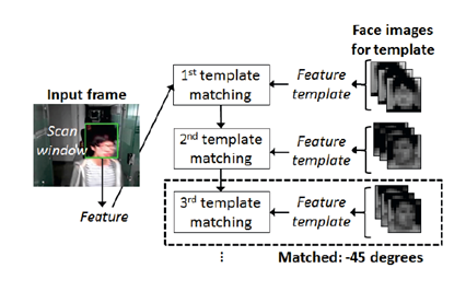
\includegraphics[scale=1]{image2-1}
  \caption{رویکرد مبتنی بر تطبیق کلیشه  \cite{ref1}.}
  \label{image2-1}
\end{figure}

\subsection{رویکردهای مبتنی بر ویژگی}
این رویکردها‌ با استخراج ویژگی‌های ساختاری چهره، چهره‌ها را پیدا می‌نمایند. ابتدا به عنوان یک طبقه‌بند، آموزش دیده و سپس برای تمایز میان نواحی شامل چهره و بدون چهره در تصویر استفاده می‌شوند. ایده این رویکرد، غلبه بر محدودیت دانش ما از چهره‌ها می‌باشد. در \cite{HJELMAS2001236} تعدادی از این رویکردها مورد بررسی قرار گرفته است:

\subsubsection{رویکرد مبتنی بر حرکت}
اگر یک توالی از چند فریم در اختیار باشد، می‌توان به کمک اطلاعات حرکت، یافتن چهره را انجام داد. برای این کار به کمک تفاصل فریم‌ها، قسمت متحرک نسبت به پس زمینه شناسایی شده و بخش بالای آن جدا می‌شود. بدین ترتیب می‌توان با احتمال بالا، مکان چهره یک فرد را در یک تصویر پیدا نمود. این رویکرد در مواجه با اجسام متحرک دیگری مانند اتومبیل دچار اشتباه می‌شود.

\subsubsection{رویکرد مبتنی بر لبه}
ابتدا به کمک یک الگوریتم لبه یاب، لبه‌های تصویر بدست می‌آید، سپس نازک سازی می‌شوند و شاخه‌های اضافه حذف می‌گردد (شکل 2-2). گوشه لبه‌ها تشخیص داده می‌شوند و هر مولفه متصل  به شاخه مرکزی آن کاهش می-یابد. اجزایی که ویژگی چهره در آن‌ها نیست حذف می‌شوند و اجزای نهایی به عنوان سمت چپ چهره، خط مو، یا سمت راست چهره برچسب گذاری می‌شوند. در یک آزمایش که 60 تصویر دارای پس زمینه پیچیده حاوی 90 چهره به این سامانه داده شده است، سامانه قادر به یافتن 76\% چهره‌ها بوده است.

\begin{figure}[h]
\centering
  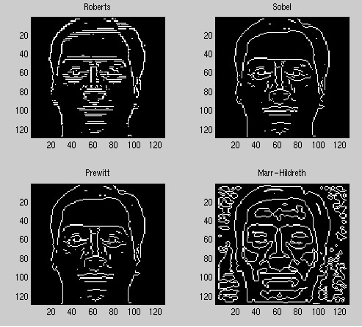
\includegraphics[scale=0.6]{image2-2}
  \caption{استفاده از لبه یاب های معروف برای استخراج ویژگی های مبتنی بر لبه از چهره  \cite{ref1}.}
  \label{image2-2}
\end{figure}

\subsubsection{رویکرد مبتنی بر اطلاعات سطح خاکستری} 
سطوح خاکستری تصویر چهره شامل اطلاعات مفیدی می‌باشد. برای مثال ابرو‌ها، مردمک چشم و لب‌ها معمولا تاریک تر از سایر نواحی صورت هستند. این ویژگی‌ها می‌تواند به یافتن یک چهره در تصویر کمک نماید. در این رویکرد ابتدا بر روی تصویر ورودی، عملیات بسط تباین  و عملیات مورفولوژی  مبتنی بر سطح خاکستری انجام می‌شود تا تصویر بهبود پیدا کند و یافتن نواحی تیره تر، راحت شود. سپس تصویر به چندین بخش تقسیم می‌شود و سطوح خاکستری بخش‌ها مورد بررسی قرار می‌گیرد. مزیت این رویکرد، کارایی در تصاویر با وضوح پایین می‌باشد (شکل 2-3).

\begin{figure}[h]
\centering
  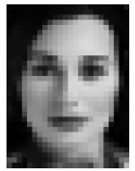
\includegraphics[scale=0.6]{image2-3}
  \caption{اطلاعات سطح خاکستری حتی در وضوح پایین نیز قابل دسترسی می باشند  \cite{ref1}.}
  \label{image2-3}
\end{figure}

\subsubsection{رویکرد مبتنی بر اطلاعات رنگی}
رنگ در تصویر اطلاعات با ارزشی به ما می‌دهد و می‌توان از رنگ پوست انسان برای یافتن چهره در تصویر استفاده کرد. برای این کار ابتدا رنگ‌ها هنجار سازی  می‌شوند تا اثر نور پردازی از بین برود. گسترده ترین فضای رنگ مورد استفاده RGB می‌باشد.
\begin{equation}\label{eq2-1}
r = \frac{R}{R + G + B}
\end{equation}

\begin{equation}\label{eq2-2}
g = \frac{G}{R + G + B}
\end{equation}

\begin{equation}\label{eq2-3}
b = \frac{B}{R + G + B}
\end{equation}

در روابط بالا \lr{R} میزان سطح رنگ قرمز، \lr{G} میزان سطح رنگ سبز و \lr{B} میزان سطح رنگ آبی در هر پیکسل از تصویر می‌باشد. 
\lr{r}
، 
\lr{g}
و
\lr{b}
به ترتیب مقدار هنجار سازی شده برای رنگ قرمز، سبز و آبی می‌باشد. واضح است که:
    
\begin{equation}\label{eq2-3}
r + g + b = 1
\end{equation}
 	
پس می‌توان فقط با داشتن مقدار \lr{r} و \lr{g} مقدار \lr{b} را بدست آورد. با توجه به بافت‌نگار  رنگ سبز و قرمز تصویر، رنگ پوست انسان، بخش کوچکی از بافت‌نگار را اشغال می‌کند. بنابراین با بررسی پیکسل‌های تصویر، می‌توان با دقت بالایی احتمال حضور چهره در تصویر را تشخیص داد و رنگ پوست انسان را می‌توان به راحتی با یک تابع گوسی تخمین زد. فضاهای رنگی دیگری نیز در این زمینه مورد استفاده قرار گرفته است. مانند
\lr{HSV},
\lr{YIQ},
\lr{YES},
\lr{YCrCb},
\lr{Lab}.
یک ایده خوب این است که وقتی شخص از دوربین فاصله زیادی دارد از رنگ پوست استفاده کنیم و وقتی شخص نزدیک به دوربین می‌باشد از ویژگی‌های قدرتمندتر چهره استفاده نماییم.

\subsection{رویکرد مبتنی بر عامل‌های آماری}
رویکرد‌های بخش‌های قبل بر روی اطلاعات استخراج شده از تصاویر چهره در شرایط آزمایشگاهی تکیه می‌کنند و اگر یک تصویر چهره در شرایط کنترل نشده و پس زمینه پیچیده داده شود، بسیاری از این رویکردها شکست می‌خورند.
استفاده از عامل‌های آماری برای ویژگی‌ها و ارائه یک مدل احتمالی برای چهره، باعث انعطاف پذیری بیشتر سامانه می-شود. این رویکرد قادر است در مواجه با جا به جایی، چرخش و تغییر مقیاس با دقت بیشتری عمل نماید. در یک رویکرد دقیق‌تر از شبکه‌های بیز  برای یافتن احتمالاتی چهره بهره گرفته شده است. یافتن چهره در حضور عینک و برخی ویژگی‌های از دست رفته نیز توسط این رویکرد انجام می‌شود.

\noindent
تا به امروز صدها رویکرد برای یافتن چهره ارائه شده است تا آن را پیشرفته تر و دقیق تر نماید، اما انقلاب الگوریتم‌های یافتن چهره در سال 2001 بود. زمانی که \lr{Viola} و \lr{Jones} در \cite{990517} یک الگوریتم چهره یاب بی‌درنگ معرفی کردند که قادر به یافتن چهره با دقت بالا بود. در ادامه به شرح این الگوریتم می‌پردازیم.

\noindent
پیش پردازش: ابتدا تصویر از فضای \lr{RGB} به تصویر سطح خاکستری تبدیل می‌شود. زیرا تشخیص چهره‌ها در تصویر خاکستری برای سامانه آسان است. سپس در صورت نیاز، پیش پردازش‌هایی مانند تغییر اندازه ، برش ، تار شدن  و تیزکردن لبه های تصویر انجام می‌شود. 

\noindent
ویژگی‌های \lr{Haar}: تمام چهره‌های انسانی ویژگی‌های مشترکی دارند. برای مثال ناحیه چشم تاریک‌تر از پیکسل‌های همسایه آن است و ناحیه بینی از چشم روشن‌تر است. ویژگی‌های \lr{Haar} مستطیل‌هایی هستند که نشان دهنده بخش‌های مختلف صورت می‌باشند. شکل ‏2-4 نمونه‌هایی از مستطیل‌های ویژگی‌های \lr{Haar} را نشان می‌دهد.
\begin{figure}[h]
\centering
  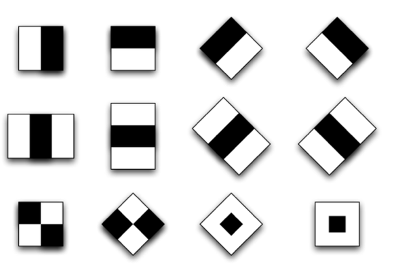
\includegraphics[scale=1]{image2-4}
  \caption{نمونه هایی از مستطیل های ویژگی های Haar \cite{ref1}.}
  \label{image2-4}
\end{figure}

\noindent
ویژگی‌های‌ \lr{Haar} برای تشخیص چشم، بینی، دهان و... با کمک تشخیص لبه، تشخیص خط و تشخیص مرکز در تصویر و استخراج ویژگی برای یافتن چهره استفاده می‌شود. مستطیل‌های ویژگی‌های \lr{Haar}، متناسب با بخش‌های چهره می‌باشند که مثالی از آن در شکل 2-5 نشان داده شده است.

\begin{figure}
\begin{subfigure}{.5\textwidth}
  \centering
  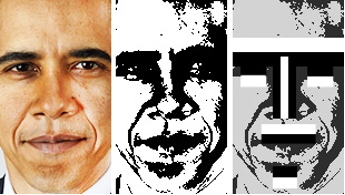
\includegraphics[scale=1]{image2-5-a}
  \label{image2-5-a}
\end{subfigure}
\begin{subfigure}{.5\textwidth}
  \centering
  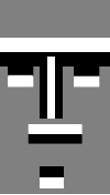
\includegraphics[scale=1]{image2-5-b}
  \label{image2-5-b}
\end{subfigure}
\caption{مستطیل های ویژگی های Haar متناسب با بخش های چهره می باشند \cite{ref1}.}
\label{fig:image2-5}
\end{figure}

\noindent
همانطور که در شکل 2-6 مشاهده می‌شود، هر مستطیل در بخش‌های مختلف چهره در روندی تکراری با اندازه‌های مختلف قرار می‌گیرد و نتیجه نهایی از کم کردن مجموع سطح روشنایی پیکسل‌های زیر بخش‌های سیاه از مجموع سطح روشنایی پیکسل‌های زیر بخش‌های سفید به دست می‌آید که یک عدد می‌باشد. از یک پنجره با اندازه ۲۴×۲۴ برای قرار دادن مستطیل‌ها بر روی تصویر استفاده می‌شود که تعداد زیاد و اندازه‌های مختلف آن‌ها باعث می‌شود برای محاسبه نتیجه نهایی نیاز به انجام بیش از ۱۶۰۰۰۰ محاسبه باشد که زمان زیادی برای هر تصویر خواهد گرفت.

\begin{figure}[h]
\centering
  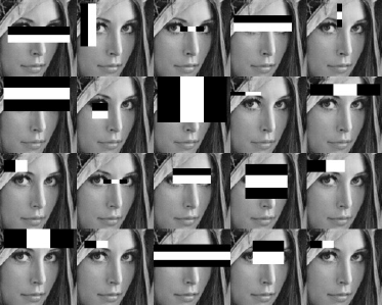
\includegraphics[scale=1]{image2-6}
  \caption{هر مستطیل در اندازه های مختلف بر روی بخش های مختلف تصویر قرار می گیرد \cite{ref1}.}
  \label{image2-6}
\end{figure}

\noindent
\lr{Ada Boost}: 
همانطور که در شکل 2-7 مشاهده می‌شود، تمام ویژگی‌های Haar برای تصویر ورودی مناسب نخواهد بود. بعضی از این ویژگی‌ها باید نادیده گرفته شوند و فقط ویژگی‌های مرتبط انتخاب شوند تا در زمان صرفه جویی شود. این کار به صورت خودکار به کمک عنصر Ada Boost انجام می‌شود.
\begin{figure}[h]
\centering
  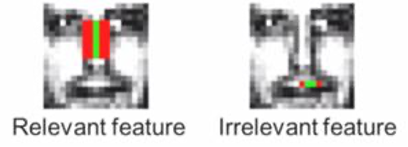
\includegraphics[scale=1]{image2-7}
  \caption{یک ویژگی مرتبط در مقابل یک ویژگی نامرتبط \cite{ref1}.}
  \label{image2-7}
\end{figure}

\noindent
\lr{Ada Boost} 
یک الگوریتم مبتنی بر یادگیری ماشین می‌باشد که ویژگی‌های کاربردی را از میان تعداد زیادی ویژگی پیدا می‌کند. بعد از شناسایی ویژگی‌های مختلف، مشخص می‌گردد که هر یک از پنجره‌ها برای بخشی از چهره مناسب می‌باشد یا خیر. هر کدام از ضرایب انتخاب شده مثبت در نظر گرفته می‌شود، در صورتی که حداقل بتواند بیش از نیمی از موارد را تشخیص دهد. این ویژگی‌ها با عنوان طبقه‌بندهای ضعیف  معرفی می‌شوند. 
\lr{Ada Boost} 
در طبقه‌بند قوی ، تعداد زيادی طبقه‌بند ضعيف را با هم ترکيب مي‌کند. رابطه کلی آن به صورت زیر می‌باشد.

\begin{equation}\label{eq2-5}
F(x)=α_1 f_1 (x)+α_2 f_2 (x)+⋯
\end{equation}

\noindent
که در آن \lr{F} طبقه‌بند قوی می‌باشد که از تعدادی f\textsubscript{i} که طبقه‌بند ضعیف می‌باشد، تشکیل شده است. هر کدام از طبقه‌بندهای ضعیف، یک خروجی صفر یا یک تولید می‌کنند. α\textsubscript{i} وزن مربوط به طبقه‌بند می‌باشد. با استفاده از این الگوریتم و وزن دادن به ویژگی‌ها، بیش از ۱۶۰۰۰۰ ویژگی قبلی به کمتر از ۲۵۰۰ ویژگی کاهش پیدا می‌کند.

\noindent
تصویر یکپارچه : تصویر یکپارچه، یا جدول محدوده مجتمع ، به منظور ارزيابی سريع‌تر ویژگی‌هایی که در بخش اول معرفی شد، استفاده می‌شود. با توجه به شکل 2-8 در یک تصویر یکپارچه مقدار پیکسل در مکان \lr{x} و \lr{y} برابر با جمع مقادیر پیکسل‌های بالا و چپ پیکسل \lr{x} و \lr{y} می‌باشد.

\begin{figure}[h]
\centering
  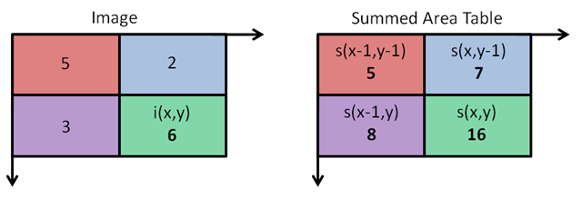
\includegraphics[scale=1]{image2-8}
  \caption{نحوه مقدار دهی به پیکسل های تصویر یکپارچه \cite{ref1}.}
  \label{image2-8}
\end{figure}

\noindent
به عنوان مثال در شکل 2-9 مقدار پیکسل‌ها به صورت زیر محاسبه می‌شود:
\begin{itemize}
\item
مقدار پیکسل ۱ در تصویر یکپارچه برابر است با مجموع پیکسل‌ها در مستطیل \lr{A}.
 \item
مقدار پیکسل ۲ در تصویر یکپارچه برابر است با مجموع پیکسل‌ها در مستطیل \lr{A} و \lr{B}.
 \item
مقدار پیکسل ۳ در تصویر یکپارچه برابر است با مجموع پیکسل‌ها در مستطیل \lr{A} و \lr{C}.
 \item
مقدار پیکسل ۴ در تصویر یکپارچه برابر است با مجموع پیکسل‌ها در مستطیل \lr{A} و \lr{B} و \lr{C} و \lr{D}.
\item
مجموع پیکسل‌ها در مستطیل \lr{D} می‌تواند به صورت (۳+۲) - (۱+۴) محاسبه شود.

\end{itemize} 


\begin{figure}[h]
\centering
  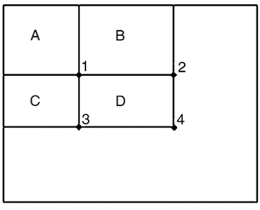
\includegraphics[scale=1]{image2-9}
  \caption{بخشی از یک تصویر که تصویر یکپارچه آن محاسبه می شود \cite{ref1}.}
  \label{image2-9}
\end{figure}

\noindent
مراحل آبشاری : اگر تصویر به مربع‌های ۲۴×۲۴ پیکسلی تقسیم شده و با پردازش هر بخش که ۲۵۰۰ ویژگی دارد، تشخیص داده شود که چهره‌ای در تصویر وجود دارد یا خیر، حجم محاسبات بسیار زیاد خواهد بود. مراحل آبشاری این فرایند را سریع‌تر انجام می‌دهد. ۲۵۰۰ ویژگی هر مربع ۲۴×۲۴ به دسته‌بندی‌های مختلف تقسیم می‌شود. برای مثال ۱۰ ویژگی در دسته‌ اول، ۲۰ ویژگی در دسته دوم، ۱۰۰ ویژگی در دسته سوم و... . می‌توان بعد از پردازش هر دسته، در ارتباط با وجود یا عدم وجود چهره در آن دسته تصمیم گرفت تا بخش‌هایی که چهره در آن وجود ندارد زودتر حذف شوند. شکل 2-10 یک نمای کلی از روند تشخیص آبشاری را نشان می‌دهد. مجموعه ای از طبقه‌بندها به هر زیر پنجره اعمال می‌شود. طبقه بند اولیه تعداد زیادی از نمونه‌های منفی را حذف می‌کند و پردازش کمی دارد. لایه‌های بعد، منفی‌های اضافی را حذف می‌کنند که نیاز به محاسبات بیشتری دارند. این الگوریتم عملکرد بسیار خوبی در برنامه‌های کاربردی بی‌درنگ و در حضور پس زمینه‌های شلوغ نشان داده است. اما هنوز در برای چهره‌هایی که رو به روی دوربین نیستند، تغییرات شدید نور، انسداد و... دارای چالش می‌باشد.

\begin{figure}[h]
\centering
  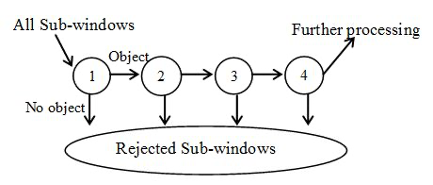
\includegraphics[scale=1]{image2-10}
  \caption{بخشی از یک تصویر که تصویر یکپارچه آن محاسبه می شود \cite{ref1}.}
  \label{image2-10}
\end{figure}

\noindent
در سال ۲۰۰۵ \lr{Dalal} و همکاران در \cite{1467360} روشی به نام بافت نگار شیب‌های جهت دار ارائه کردند که به اختصار \lr{HOG} نامیده می‌شود. در این روش ابتدا تصویر خاکستری می‌شود، زیرا نیازی به رنگ نیست. پیرامون هر پیکسل بررسی می‌شود تا مشخص شود نسبت به پیکسل‌های پیرامونش چقدر تاریک می‌باشد. مطابق شکل 2-11 جهتی انتخاب می‌شود که به سمت پیکسل‌های تاریکتر باشد. این روند برای همه پیکسل‌های تصوير انجام می‌شود و به ازای هر پیکسل یک جهت ذخیره خواهد شد که روندی از روشنايى به تاريكى را در تصوير نمايش مي‌دهند.

\begin{figure}
\begin{subfigure}{.5\textwidth}
  \centering
  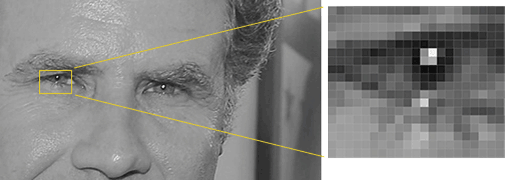
\includegraphics[scale=1]{image2-11-a}
  \label{image2-11-a}
\end{subfigure}
\begin{subfigure}{.5\textwidth}
  \centering
  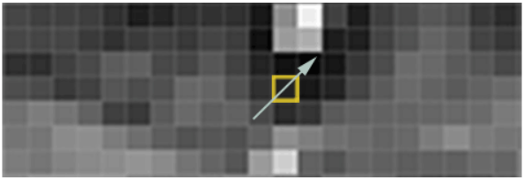
\includegraphics[scale=1]{image2-11-b}
  \label{image2-11-b}
\end{subfigure}
 \caption{سطح روشنایی پیکسل های اطراف هر پیکسل بررسی شده و راستای روشن به سمت تاریک برگزیده می شود \cite{ref1}.}
\label{fig:image2-11}
\end{figure}

\noindent
دليل استفاده از جهت‌ها این است که اگر پیکسل‌ها به طور مستقيم استفاده شوند، تصوير تاريك و تصوير روشن از يك چهره مشخص، دارای سطح روشنایی متفاوتى خواهند بود. اما با در نظر گرفتن جهتى تغییر روشنايى، هم تصوير تيره و هم تصوير روشن، نمايش يكسانى خواهند داشت كه حل مسئله را آسان‌تر مي‌كند.
ذخيره جهت‌ها براى تمام پیکسل‌ها باعث افزایش جزئيات می‌شود. لذا روند اصلى روشنايى و تاريكى در سطحی بالاتر در نظر گرفته می‌شود، به طورى كه بتوان الگوى اصلى تصوير را ديد. تصوير به بخش‌هاى ١٦×١٦ پيكسل تقسیم می-شود و در هر بخش تعداد جهت‌هاى به سمت بالا، پايين، چپ و راست شمارش مي‌شود. سپس بخش‌هاى درون تصوير با جهت‌هايى كه بزرگتر بودند، جايگزين مي‌شود. نتيجه نهايى، تبديل تصوير به يك نمايش ساده شده از ساختار چهره است که در شکل 2-12 مشاهده می‌شود. براى يافتن چهره‌ها در این الگوریتم، بخش‌هايى از تصوير كه به الگوى \lr{HOG} شبيه‌تر است، مشخص می‌شود. با استفاده از اين روش، مي‌توان چهره‌ها را در تصویر به سادگى پيدا كرد.

\begin{figure}
\begin{subfigure}{.5\textwidth}
  \centering
  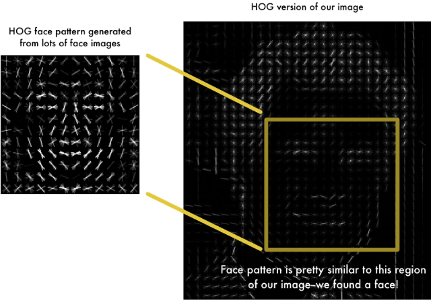
\includegraphics[scale=1]{image2-12-a}
  \label{image2-12-a}
\end{subfigure}
\begin{subfigure}{.5\textwidth}
  \centering
  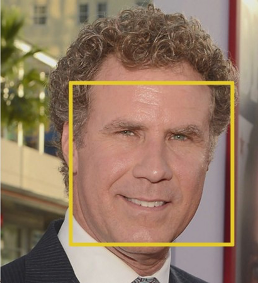
\includegraphics[scale=1]{image2-12-b}
  \label{image2-12-b}
\end{subfigure}
  \caption{براى يافتن چهره ها، بخش هايى از تصوير كه به الگوى HOG شبيه تر است را پيدا می كنيم \cite{ref1}.}
\label{fig:image2-12}
\end{figure}

در سال 2015 \lr{Shengcai Liao} و همکاران در \cite{7130626} یک روش دقیق و سریع برای یافتن چهره ارائه دادند که در آن از اختلاف پیکسل هنجارسازی شده یا \lr{NDP} برای یافتن چهره استفاده می‌شود. ارزیابی ویژگی \lr{NPD} بسیار سریع است و دسترسی به حافظه تنها با استفاده از یک جدول جستجو می‌باشد. در این روش نشانه گذاری یا خوشه بندی در مرحله آموزش نیز لازم نیست و در برابر تغییرات نور، حالت، انسداد، تصاویر با وضوح پایین و... مقاوم است. \lr{NPD} بین دو پیکسل در یک تصویر به صورت زیر تعریف شده است:
\begin{equation}\label{eq2-6}
f(x,y) = \frac{x - y}{x + y}
\end{equation}

\noindent
که در آن \lr{x} و \lr{y} بزرگتر از صفر هستند و \lr{f(0,0)} برای حالتی که \lr{x = y = 0} باشد، برابر صفر است. این عمل بر روی هر جفت پیکسل از تصویر اجرا می‌شود. اگر تصویر ورودی مربعی با ابعاد \lr{s} باشد و \lr{p=s×s} تعداد پیکسل‌ها باشد، آنگاه تعداد ویژگی‌های استخراج شده برابر \lr{d=p(p-1)/2} می‌باشد. سپس علامت  ویژگی‌های استخراج شده مورد استفاده قرار می‌گیرد که وابسته به اندازه سطح روشنایی پیکسل‌ها نمی‌باشد. بلکه تنها نشان می‌دهد کدام ناحیه روشن‌تر و کدام ناحیه تیره‌تر می‌باشد. همچنین این ویژگی‌ها به خدشه حساس نمی‌باشند. در نهایت ویژگی‌های استخراج شده به عنوان ورودی به یک سامانه یادگیری داده می‌شود. نمونه‌ای از نتیجه اجرای این الگوریتم بر روی مجموعه داده \lr{FDDB} در شکل 2-13 آمده است.
 
 \begin{figure}[h]
\centering
  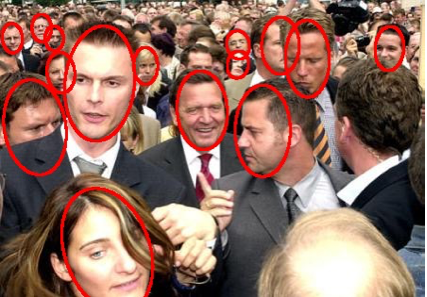
\includegraphics[scale=1]{image2-13}
  \caption{نتیجه اجرای روش مبتنی بر NPD \cite{ref1}.}
  \label{image2-13}
\end{figure}

\noindent
تمام رویکرد‌های ارائه شده که یافتن چهره را با مدل سازی صریح از ویژگی‌های صورت انجام می‌دهند، در برابر تغییرات غیر قابل پیش بینی چهره و شرایط محیطی دچار مشکل می‌شوند. اگرچه بعضی از تلاش‌های اخیر مبتنی بر ویژگی، توانایی مقابله با شرایط کنترل نشده را بهبود داده اند، اما بیشتر آن‌ها هنوز به چهره‌های رو به رو و شرایط کنترل شده محدود می‌شوند، و به عنوان یکی از روش‌های یک سامانه ترکیبی در نظر گرفته شده اند. پس نیاز به روش-هایی هست که بتوانند در شرایط خصمانه تر مانند تشخیص چهره‌های متعدد در زمینه‌های شلوغ به خوبی عمل کنند.

 \subsection{رویکردهای مبتنی بر تصویر}
رویکردهای مبتنی بر تصویر نیاز به مجموعه‌ای از تصاویر آموزشی برای پیدا کردن مدل‌های چهره دارند و بر اساس استخراج ویژگی و یادگیری ماشین عمل می‌نمایند. مجموعه‌ای از تصویر‌های مختلف چهره طبقه‌بندی می‌شوند و برای تشخیص چهره جدید از این طبقه‌بندی استفاده می‌شود. نمونه‌هایی از چهره و نمونه‌هایی از غیر چهره به طبقه‌بند داده می-شود تا از روی این تصویرها عمل یادگیری انجام شود. به طور تجربی دقت نتایج رویکردهای مبتنی بر تصویر بهتر از سایر رویکرد‌ها می‌باشد. این رویکردها به چند دسته تقسیم می‌شوند که در ادامه شرح داده شده است. 

 \subsubsection{رویکرد مبتنی بر ماشین بردار پشتیبان}
ماشین‌ بردار پشتیبان  طبقه‌بندی خطی می‌باشد که حاشیه بین ابرصفحه تصمیم و داده‌های آموزش را به حداکثر می-رساند. برای اولین بار در سال 1997 \lr{Osuna} و همکاران در \cite{609310} از این طبقه‌بند برای یافتن چهره استفاده کردند.

 \subsubsection{رویکرد مبتنی بر شبکه‌ عصبی}
یک راه حل غیر خطی برای یافتن چهره، استفاده از شبکه‌های عصبی است. اولین رویکردهای عصبی در یافتن چهره بر اساس \lr{MLP} بود که در مجموعه داده‌های ساده، امیدوار کننده بود. شبکه‌های عصبی با معماری پیمانه ای  امروزی بسیار پیچیده‌تر از \lr{MLP} ساده هستند. نوع خاصی از شبکه‌های عصبی عمیق برای پردازش تصاویر استفاده می‌شوند که شبکه عصبی پیچشی  نام دارند. ساختار عمیق این شبکه‌ها باعث شد در مجموعه داده‌های بزرگ و دشوار نتایج خوبی بدست آید. شکل ‏2-14 نمای کلی یک شبکه عصبی پیچشی برای یافتن چهره را نشان می‌دهد. یک شبکه عصبی پیچشی از تعدادی تابع و لایه تشکیل شده است. لایه‌های شبکه عصبی عبارتند از:

\noindent
لایه‌های پیچشی  برای لغزاندن یک پنجره بر روی ورودی

\noindent
لایه‌های تمام متصل  برای محاسبه مجموع وزن دار تمام واحد های ورودی

\noindent
لایه‌های رای گیری  به منظور کاهش حجم داده‌ها با محاسبه مقدار بیشینه، میانگین یا اندازه اقلیدسی هر بخش
 
\begin{figure}[h]
\centering
  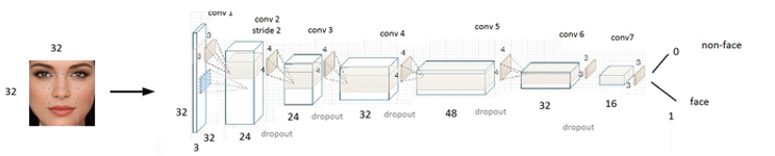
\includegraphics[scale=1]{image2-14}
  \caption{نمای کلی یک شبکه عصبی پیچشی برای یافتن چهره \cite{ref1}.}
  \label{image2-14}
\end{figure}

\noindent
با توجه به آنچه در \cite{8253595} آمده است، چالش اصلی در یافتن چهره این است که ویژگی‌هایی مانند \lr{Haar} و \lr{HOG} اطلاعات برجسته چهره را در شرایط مختلف نما، نورپردازی، رنگ پوست، انسداد، استفاده از لوازم آرایشی و... استخراج نمی‌کنند. این محدودیت بیشتر به دلیل ویژگی‌های استفاده شده در طبقه‌بندها است. با پیشرفت‌های اخیر در رویکردهای یادگیری عمیق و در دسترس بودن پردازنده‌های گرافیکی، استفاده از شبکه‌های عصبی پیچشی عمیق برای استخراج ویژگی امکان پذیر شده است. ویژگی‌های عمیق به دست آمده به طور گسترده‌ای برای یافتن چهره استفاده می‌شود. با توجه به شکل 2-15 روش‌های مبتنی بر شبکه عصبی پیچشی عمیق برای یافتن چهره به دو زیر شاخه تقسیم می‌شود: رویکرد مبتنی بر ناحیه و رویکرد پنجره لغزان.

\begin{figure}[h]
\centering
  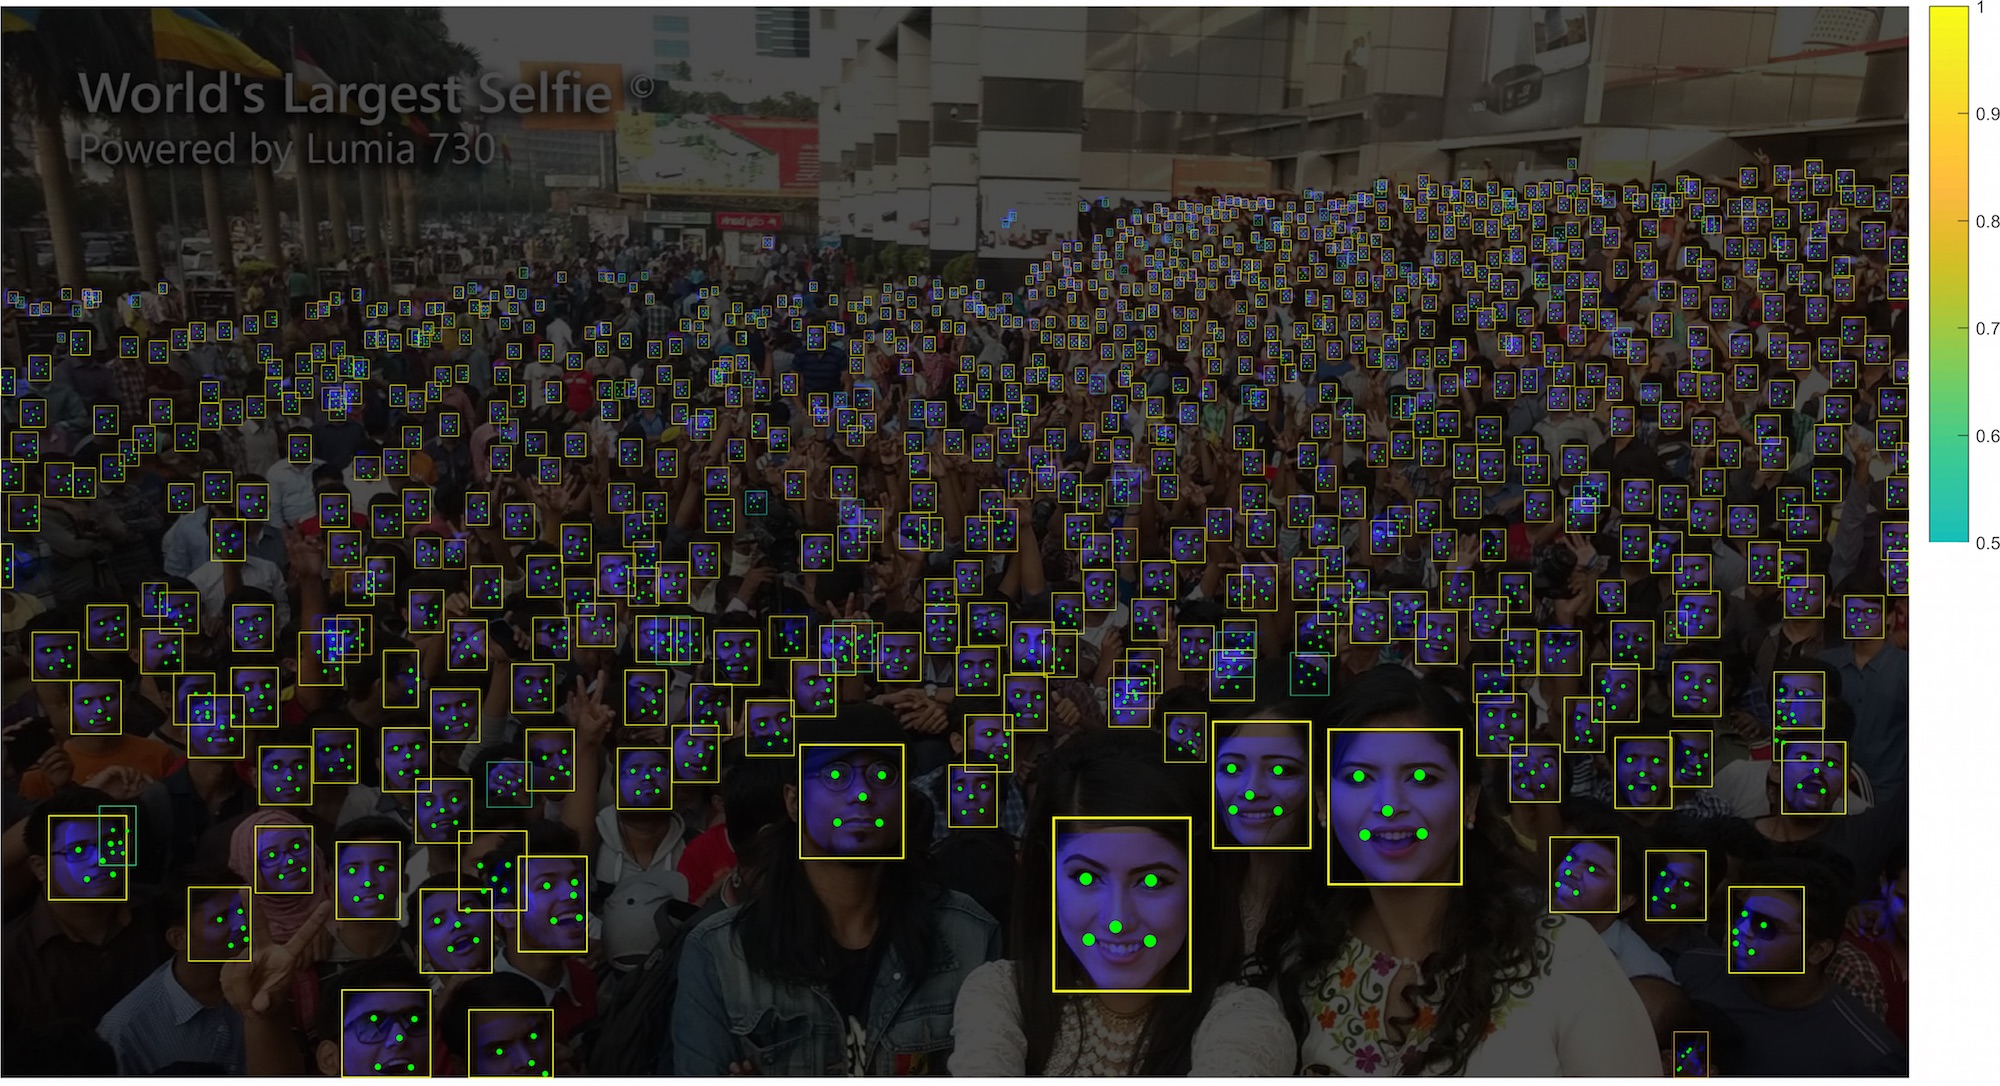
\includegraphics[scale=1]{image2-15}
  \caption{یافتن چهره مبتنی بر شبکه عصبی عمیق (a) رویکرد مبتنی بر ناحیه و (b) رویکرد پنجره لغزان \cite{ref1}.}
  \label{image2-15}
\end{figure}

\section{شناسایی چهره}
شناسایی چهره در دو مرحله انجام می‌شود. مرحله اول استخراج ویژگی و مرحله دوم، طبقه‌بندی است. الگوریتم‌های شناسایی چهره را می‌توان به دو دسته اصلی تقسیم کرد. الگوریتم‌های هندسی که بر مبنای استخراج ویژگی‌های متمایز چهره‌ها کار می‌کنند، و الگوریتم‌های تصویری که تصویر را تبدیل به یک الگو می‌نماید و الگوها را مقایسه می‌نماید. رویکردهای مختلفی برای شناسایی چهره طراحی شده است که در ادامه مهم‌ترین آن‌ها آمده است.

\subsection{رویکرد‌های سنتی}
این رویکردها ویژگی‌های چهره را با علامت‌ها و اندازه‌ها از تصویر استخراج می‌کنند. برای مثال موقعیت نسبی، اندازه و یا شکل چشم‌ها، بینی، گونه‌‌ها و فک را محاسبه کرده و تجزیه و تحلیل می‌کنند. سپس از این ویژگی‌ها برای جستجوی تصاویر دیگر در پایگاه داده استفاده می‌کنند. در سال 1993 \lr{Roberto Brunelli} و همکاران در \cite{254061} یکی از اولین الگوریتم‌ها در این زمینه را ارائه دادند که رویکرد‌ موفقی مبتنی بر روش‌های تطبیق الگو داشت (شکل 2-16). این رویکرد در شرایط کنترل شده به دقت 90\% رسید.
 
 \begin{figure}[h]
\centering
  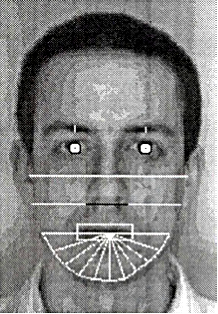
\includegraphics[scale=1]{image2-16}
  \caption{ویژگی های هندسی (رنگ سفید) مورد استفاده در آزمایش های تشخیص چهره \cite{ref1}.}
  \label{image2-16}
\end{figure}

\subsection{رویکرد مبتنی بر فیلتر گابور ‌}
همانطور که در \cite{ABATE20071885} آمده است، در این رویکرد ابتدا تصویر را بخش بندی کرده، سپس بر روی بخش‌های مختلف آن، فیلتر گابور اعمال می‌شود و نتیجه بدست آمده با یک طرح از پیش آماده شده، با یک آستانه گذاری مطابقت داده می‌شود. شکل 2-17 فیلترهای چندگانه گابور و تاثیر این فیلترها بر روی تصویر چهره انسان را نشان می‌دهد. دلیل استفاده از فیلتر گابور این است که عملکرد این فیلتر به سامانه بصری انسان بسیار شباهت دارد. 
 	 
\begin{figure}
\begin{subfigure}{.5\textwidth}
  \centering
  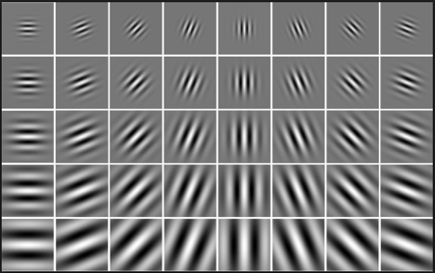
\includegraphics[scale=1]{image2-17-a}
  \label{image2-17-a}
\end{subfigure}
\begin{subfigure}{.5\textwidth}
  \centering
  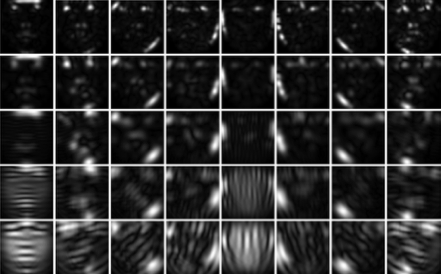
\includegraphics[scale=1]{image2-17-b}
  \label{image2-17-b}
\end{subfigure}
  \caption{(الف) فیلترهای چندگانه گابور (ب) تاثیر این فیلترها بر روی تصویر چهره \cite{ref1}.}
\label{fig:image2-17}
\end{figure}

\subsection{رویکرد‌های سه بعدی}
همانطور که در \cite{10.3745/JIPS.2009.5.2.041} آمده است، داده‌های سه بعدی دقت تشخیص چهره را به شدت بهبود می‌بخشد، اختلاف داده‌های ورودی با داده‌های ذخیره شده زیادتر است و سامانه با دقت بیشتری عمل می‌کند. روش تشخیص سه بعدی چهره از یک منتشر کننده نور فرو سرخ و یک حسگر به عنوان دریافت کننده استفاده می‌کند. شبکه‌ای از نورهای فرو سرخ که برای انسان قابل رویت نیست، روی چهره تابانده می‌شود. سپس یک حسگر ویژه، پرتوهای بازتاب را دریافت کرده و اطلاعات عمق تصویر پردازش می‌شود. این دسته از الگوریتم‌ها برای شناسایی دقیق اشخاص، برای هر نفر برداری‌های سه بعدی می‌سازند. عیب رویکردهای سه بعدی، نیاز به تجهیزات پیشرفته و غیر قابل استفاده بودن در شرایط کنترل نشده مانند خیابان و معابر پیاده می‌باشد. شکل 2-18 یک مدل سازی سه بعدی چهره با اشعه فروسرخ را نشان می‌دهد.

\begin{figure}[h]
\centering
  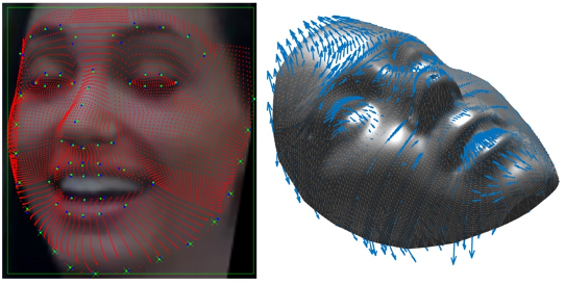
\includegraphics[scale=1]{image2-18}
  \caption{مدل سازی سه بعدی چهره با اشعه فرو سرخ \cite{ref1}.}
  \label{image2-15}
\end{figure}
 
 \subsection{رویکرد‌های تجزیه و تحلیل بافت پوست}
یکی دیگر از رویکردهای در حال ظهور، استفاده از بافت پوست برای شناسایی چهره می‌باشد که خطوط، الگوها و لکه-های پوست را به یک فضای ریاضی تبدیل می‌کند. تجزیه و تحلیل بافت بسیار شبیه روش شناسایی چهره است. تصویری از پوست گرفته می‌شود و به بخش‌های کوچکتر تقسیم می‌شود. سپس هر بخش به یک فضای ریاضی قابل اندازه گیری تبدیل می‌شود و خطوط، منافذ و بافت پوست تشخیص داده می‌شود. این رویکرد می‌تواند تفاوت بین دوقلوهای یکسان را شناسایی کند که با استفاده از تشخیص چهره به تنهایی امکان پذیر نیست. آزمایش‌ها نشان دادند که با افزودن تحلیل بافت پوست، عملکرد سامانه تشخیص چهره می‌تواند 20 تا 25 درصد افزایش یابد.

\noindent
در سال 2017 \lr{Guosheng Hu} و همکاران در \cite{HU2017366} یک روش سه بعدی برای توصیف ویژگی‌های چهره ارائه کردند که در آن از مدل سازی سه بعدی چهره به همراه تجزیه و تحلیل بافت پوست استفاده شده است. این سامانه شایستگی استفاده در کاربردهای مختلف امنیتی و نظامی با شناسایی خودکار سریع و بدون دخالت شخص را دارد و سرعت پردازش را بالا و خطا را کاهش داده است. برتری روش سه بعدی در عدم وابستگی به حرکت و جا به جایی صورت است. انتقال و نصب سامانه تصویر برداری بسیار ساده است. زاویه دید حسگر چندان مهم نیست. همچنین نورپردازی نامناسب تاثیری در این شیوه ندارد و عملیات آن ساده است.
بر خلاف روش تشخیص دو بعدی، روش سه بعدی و تجزیه و تحلیل بافت پوست به تجهیزات بسیار پیچیده تری نیاز دارد، و با توجه به آنکه تمرکز ما بر روی تشخیص چهره به صورت بی‌درنگ در شرایط کنترل نشده مانند معابر پیاده و خیابان می‌باشد، به توضیح مختصر رویکردهای سه بعدی و تجزیه و تحلیل بافت پوست بسنده می‌کنیم.

 \subsection{رویکرد‌های مبتنی بر دوربین حرارتی}
در این رویکرد، دوربین حرارتی شکل صورت را تشخیص می‌دهد و از لوازم جانبی مانند عینک، کلاه یا آرایش چشم پوشی می‌کند. بر خلاف دوربین‌های معمولی، دوربین‌های حرارتی می‌توانند تصاویر را حتی در شرایط کم نور مانند شب، بدون استفاده از فلاش و قرار گرفتن در معرض مستقیم دوربین ضبط کنند. با این حال، یکی از مشکل‌های استفاده از تصاویر حرارتی برای تشخیص چهره این است که مجموعه داده‌های آن برای شناسایی چهره محدود است.

\noindent
در سال 2003 \lr{Diego Socolinsky} و همکاران در \cite{SOCOLINSKY200372} از شناسایی چهره مبتنی بر دوربین حرارتی در کاربردهای واقعی بهره برداری کردند و یک مجموعه داده جدید از تصاویر حرارتی چهره ایجاد کردند. آن‌ها از حسگرهای الکتریکی فروسرخ با حساسیت کم و با توانایی جذب حرارت طولانی مدت یا \lr{LWIR} استفاده کردند.
نتایج نشان می‌دهد که تلفیق \lr{LWIR} و دوربین‌های معمولی، نتایج بهتری در شرایط کنترل نشده دارد. در این مطالعه 240 چهره مجزا در طی 10 هفته برای ایجاد پایگاه داده جدید استفاده شده است. داده‌ها در روزهای آفتابی، بارانی و ابری جمع آوری شد. در شرایط کنترل شده دوربین معمولی دقت 97.05\% دارد، در حالی که روش \lr{LWIR} دارای دقت 93.93\% می‌باشد و ترکیب این دو دارای دقت 98.40\% است. در شرایط کنترل نشده دوربین معمولی دقت 67.06\%، دوربین \lr{LWIR} دقت 83.03\% و ترکیب این دو دارای دقت 89.02\% است.

 \subsection{تشخیص چهره مبتنی بر ویدیو}
در سال 2009 \lr{Huafeng Wang} و همکاران در \cite{wang2009video} یک برآورد کلی از رویکردهای مبتنی بر ویدیو ارائه دادند. تشخیص چهره در ویدیو در طی چند سال گذشته مورد توجه قرار گرفته و طیف گسترده‌ای از برنامه‌های کاربردی تجاری و اجرای قانون را در بر گرفته است. فیلم‌ها قادر به ارائه اطلاعات بیشتر نسبت به تصاویر ثابت هستند. مزایای عمده استفاده از ویدیو عبارتند از:

\begin{enumerate}
\item
	امکان استفاده از افزونگی موجود در توالی ویدیو برای بهبود عملکرد تشخیص نسبت به تصاویر ثابت وجود دارد. تشخیص چهره و پیگیری آن در طول زمان، موجب انتخاب فریم‌های خوب می‌شود که حاوی چهره‌های رو به رو یا نشانه‌های ارزشمند است که شرایط نور، انسداد، حالت چهره و... در آن رضایت بخش می‌باشد.
\item 
	مطالعات روان پزشکی نشان داده است که اطلاعات پویا در فرایند تشخیص فرد بسیار حائز اهمیت است. 
\item
	نمایش‌های موثرتر مانند مدل چهره سه بعدی یا تصاویر \lr{super resolution} می‌توانند از اطلاعات فریم‌های ویدیو گرفته شده برای بهبود شناخت استفاده کنند.
\item
	یادگیری و به روز رسانی مدل در طول زمان امکان پذیر می‌باشد.
\end{enumerate}
	
\noindent
برای تشخیص چهره در تصاویر ویدیویی، دو رویکرد کلی وجود دارد:

\noindent
مبتنی بر قاب : در این رویکرد برای شناسایی چهره، هر قاب به صورت جداگانه مورد پردازش قرار می‌گیرد که عیب آن نادیده گرفتن اطلاعات زمانی ارائه شده توسط توالی ویدیویی می‌باشد. 

\noindent
یافتن و ردیابی : یافتن چهره در اولین قاب و سپس ردیابی آن از طریق توالی قاب‌ها. شکل 2-19 نمای کلی این رویکرد را نشان می‌دهد.
 
 \begin{figure}[h]
\centering
  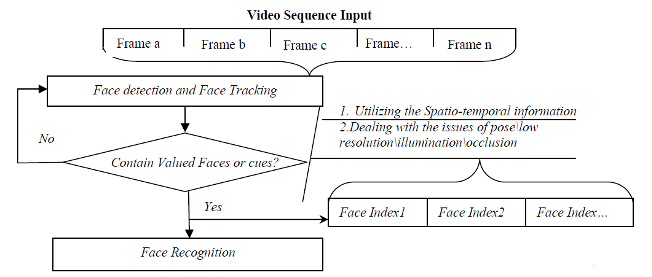
\includegraphics[scale=1]{image2-19}
  \caption{نمای کلی یک سامانه تشخیص چهره مبتنی بر ویدیو \cite{ref1}.}
  \label{image2-19}
\end{figure}

 \subsection{رویکرد مبتنی بر چهره ویژه}
با افزایش حجم داده‌های موجود، نیاز به کاهش ابعاد داده‌ها می‌باشد. تحلیل مؤلفه‌های اساسی یا \lr{PCA} یک روش‌ کاهش ابعاد داده‌ها است که در برخی مسئله‌ها مانند پردازش تصویر به خوبی و با سرعت بالا عمل می‌کند. استفاده از این روش در پردازش سریع تر داده‌ها کمک می‌کند و از رخ دادن مشکل بیش‌برازاندن  جلوگیری می‌نماید. اگر یک پایگاه داده عظیم از تصاویر چهره اشخاص با وضوح بالا موجود باشد که هر کدام دارای تعدادی زیاد ویژگی هستند، و بخواهیم یک تصویر آزمایش را با این پایگاه داده مقایسه کرده و شخص شبیه به آن را پیدا کنیم، مقایسه تصاویر بسیار زمان بر و در مواردی غیر ممکن خواهد بود. \lr{PCA} در این مسئله به خوبی عمل می‌کند. با اعمال تکنیک کاهش بعد به تصویر و با به دست آوردن تصویر ویژه چهره‌ها می‌توان ویژگی‌ها را کاهش داد و نتیجه مطلوب را در زمان بسیار کم گرفت. شکل 2-20 تعدادی چهره و چهره‌های ویژه متناظر با آن‌ها را نشان می‌دهد.

\noindent
در سال 2014 \lr{Xiao Luan} و همکاران در \cite{LUAN2014495} یک روش تشخیص چهره مبتنی بر \lr{PCA} ارائه دادند که تا حدی در برابر تغییرات نورپردازی و انسداد مقاوم می‌باشد. \lr{PCA} راستای بیشترین تغییرات را با توجه به تعداد ویژگی‌ها و نوع آن‌ها به ما می‌دهد. به همین دلیل در برخی موارد که تنها محوری که بیشترین تغییرات یا پراکندگی را دارد برای ما مهم است، راه حل مناسبی خواهد بود. 

\begin{figure}
\begin{subfigure}{.5\textwidth}
  \centering
  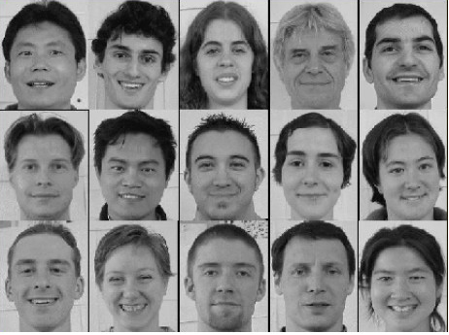
\includegraphics[scale=1]{image2-20-a}
  \label{image2-20-a}
\end{subfigure}
\begin{subfigure}{.5\textwidth}
  \centering
  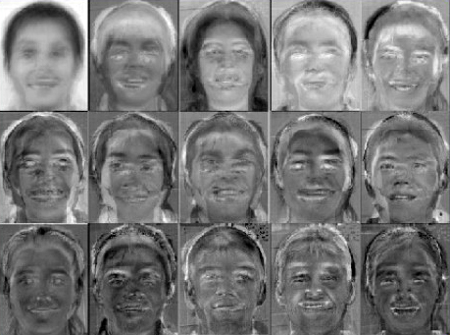
\includegraphics[scale=1]{image2-20-b}
  \label{image2-20-b}
\end{subfigure}
  \caption{ (الف) تعدادی چهره و (ب) چهره های ویژه متناظر با آن ها \cite{ref1}.}
\label{fig:image2-20}
\end{figure}

\noindent
در سال 2016 \lr{K. R. Sreelakshmi} و همکاران در \cite{7854053} یک روش شناسایی چهره مبتنی بر چهره‌های ویژه ارائه دادند که در آن ابتدا تصویر ورودی با استفاده از ماتریس بردارهای ویژه، به فضای دیگری منتقل می‎شود، سپس در فضای کاهش بعد یافته با داده‏های موجود مقایسه شده و شبیه‎ترین تصویر به آن انتخاب می‎شود. برای مقایسه از معیارهایی مانند معیار اقلیدسی و منهتن می‏توان استفاده کرد. از مزایای این روش می‏توان به سهولت پیاده‏سازی و استفاده، کاهش حجم داده‏ها و سرعت بالا اشاره کرد. در نظر نگرفتن پراکندگی درون کلاسی و بین کلاسی داده‏ها و عدم توجه به برچسب تصویر برای شناسایی و تمایز قایل نشدن بین تصاویر مختلف یک شخص در پایگاه و نیاز به بروز رسانی تمامی اطلاعات موجود با ورود یک تصویر جدید به پایگاه داده از معایب این روش است. 
محاسبات ریاضی و مراحل انجام آن‌ها:
\begin{enumerate}
\item
	تبدیل ماتریس تصاویر به بردار و کنار هم قرار دادن آن‌ها برای تشکیل ماتریس داده‏ها
\item 
	محاسبه‏ میانگین ماتریس بدست آمده و انتقال داده‏ها به مرکزیت صفر
\item
محاسبه‏ ماتریس کوواریانس بردارها و مقادیر ویژه‏ آن
\item
انتقال ماتریس داده‏ها به زیرفضای جدید با استفاده از ماتریس بردارهای ویژه
\item
	بررسی شباهت بین بردار منتقل شده و بردارهای موجود و انتخاب شبیه‏ترین بردار
\end{enumerate}

\subsection{رویکرد مبتنی بر ماشین بردار پشتیبان}
همان طور که در بخش 2-2-4-1 گفته شد، ماشین‌های بردار پشتیبان، طبقه‌بندهای خطی هستند که حاشیه بین ابرصفحه تصمیم و نمونه‌های مجموعه آموزش را به حداکثر می‌رسانند. در سال 2012 \lr{N.M.Khan} و همکاران در \cite{KHAN201266} این طبقه‌بند را برای تشخیص چهره مورد استفاده قرار دادند. یک نسخه مبتنی بر هسته برای \lr{SVM} معرفی شده که \lr{KSVM} نام گذاری شده است.

\begin{equation}\label{eq2-7}
a = b
\end{equation}

\noindent	
که در آن \lr{w} بردار وزن‌ها، \lr{x} داده‌های ورودی و \lr{w0} مقدار پیش قدر می‌باشد. سپس یک مدل بی پارامتر از \lr{LDA} به نام \lr{NDA} معرفی شده، سپس یک نسخه مبتنی بر هسته  به نام \lr{KNDA} معرفی شده است. 

\begin{equation}\label{eq2-8}
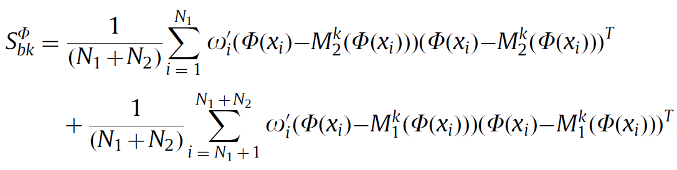
\includegraphics[height=3cm]{equation2-8}
\end{equation}

\noindent
که در آن \lr{N1} و \lr{N2} تعداد نمونه‌های آموزشی در هر دسته می‌باشند. سپس از ترکیب دو رویکرد فوق، مدلی به نام \lr{SVM + NDA} طراحی نموده است. 
\begin{equation}\label{eq2-9}
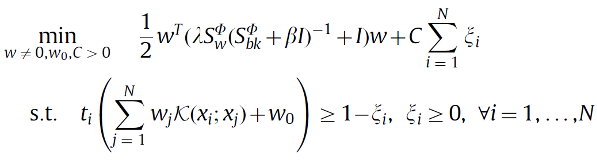
\includegraphics[height=3cm]{equation2-9}
\end{equation}	

\noindent
که در آن \lr{βI} ماتریس تنظیم می‌باشد و \lr{λ} ضریبی برای تنظیم کنترل میان \lr{SVM} و \lr{NDA} می‌باشد. رابطه بالا یک مسئله بهینه سازی می‌باشد که به صورت تکراری قابل حل ‌می‌باشد. دقت این روش در مقایسه با سایر روش‌های مشابه در جدول 2-1 آورده شده است.

\begin{table}
  \caption{ مقایسه دقت الگوریتم SVM + NDA با سایر رویکرد های مشابه}
  \label{tbl:2-1}
  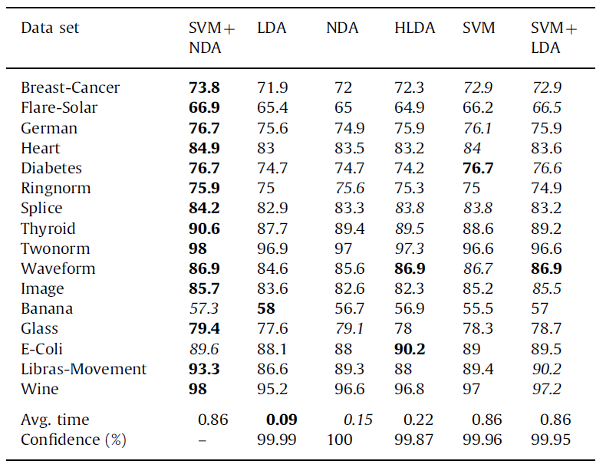
\includegraphics[width=\linewidth]{table2-1}
\end{table}
 
\subsection{رویکردهای مبتنی بر شبکه عصبی}
یک راه حل غیر خطی برای شناسایی چهره، استفاده از شبکه‌ عصبی پیچشی است که به طور شگفت انگیزی در طبقه-بندی تصاویر چهره خوب کار می‌کند و ویژگی‌های ارزشمندی را از تصویر چهره استخراج می‌کند. بنابراین می‌توان از آن در حل مسئله شناسایی چهره‌ و تأیید هویت استفاده کرد. شکل 2-21 ساختار کلی یک شبکه عصبی عمیق برای شناسایی چهره را نشان می‌دهد.
 
\begin{figure}[h]
\centering
  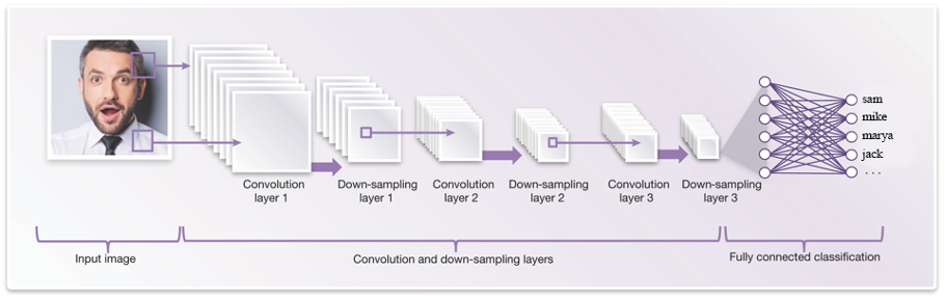
\includegraphics[scale=1]{image2-21}
  \caption{شبکه عصبی عمیق برای شناسایی چهره \cite{ref1}.}
  \label{image2-21}
\end{figure}

\noindent
معمولا به عنوان تابع فعالیت از توابع غیرخطی مانند \lr{ReLU} استفاده می‌شود. و عملیات بهینه سازی به روش پس انتشار خطا انجام می گردد. و در لایه خروجی از تابع \lr{SoftMax} برای طبقه‌بندی استفاده می‌شود که خروجی های لایه آخر را هنجار می‌کند. شبکه‌های عصبی پیچشی ویژگی‌های یک چهره را استخراج می‌کنند که می‌توان به عنوان یک شناسه برای یک فرد خاص در نظر گرفت. هنگامی که دو تصویر مختلف از چهره یک شخص به عنوان ورودی داده می‌شود، شبکه باید خروجی‌های مشابه (ویژگی‌های نزدیک تر) را برای هر دو تصویر تولید نماید، در حالی که برای چهره دو شخص مختلف، شبکه باید خروجی‌های بسیار متفاوت برای دو تصویر تولید نماید. شبکه عصبی نیاز به آموزش دارد تا به طور خودکار ویژگی‌های مختلف چهره‌ها را شناسایی کند و بر اساس آن محاسبات را انجام دهد. در ادامه چند شبکه عصبی پیچشی معروف مورد بررسی قرار گرفته است.

\subsubsection{	شبکه \lr{FaceNet}}
در سال 2015 \lr{Florian Schroff} و همکاران در \cite{7298682} یک شبکه عصبی عمیق به نام \lr{FaceNet} ارائه دادند. \lr{FaceNet} یک مدل یکپارچه است که می‌آموزد چگونه تصاویر چهره را به یک فضای اقلیدسی فشرده نگاشت دهد تا فاصله تصاویر به طور مستقیم با میزان شباهت چهره‌ها مرتبط باشد. هنگامی که این فضا تولید شود، شناسایی چهره، تایید هویت و خوشه‌بندی می‌تواند به راحتی با استفاده از روش‌های استاندارد توسط \lr{FaceNet} انجام شود. این شبکه برای آموزش از سه گانه تطبیق – عدم تطبیق استفاده می‌نماید. با توجه به شکل 2-22، سه گانه تطبیق – عدم تطبیق یک مجموعه از سه تصویر شامل یک تصویر مرجع، یک تصویر منطبق بر تصویر مرجع و یک تصویر غیر منطبق بر تصویر مرجع است که باید فاصله بین تصویر مرجع و تصویر منطبق را به حداقل برساند، زیرا هر دو دارای هویت مشابه هستند و فاصله بین تصویر مرجع و تصویر غیر منطبق را به حداکثر برساند، زیرا این تصاویر دارای هویت متفاوت می‌باشند. 
 
 \begin{figure}[h]
\centering
  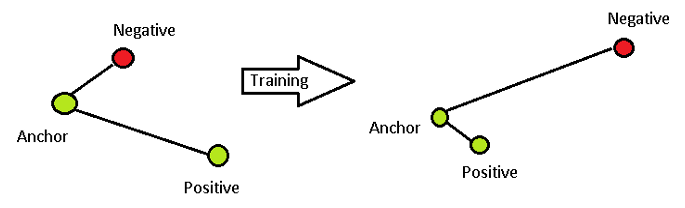
\includegraphics[scale=1]{image2-22}
  \caption{سه گانه تطبیق – عدم تطبیق \cite{ref1}.}
  \label{image2-22}
\end{figure}

\noindent 
برای هر داده آموزشی \lr{A} مجموعه‌ای از داده‌های مشابه \lr{Positive} و مجموعه‌ای از داده‌های نامرتبط \lr{Negative} در نظر گرفته می‌شود. سپس داده‌ها با تابع ضرر سه گانه طوری آموزش می‌بینند که رابطه زیر برای هر کدام از داده‌های آموزشی برقرار باشد.
\begin{equation}\label{eq2-10}
‖f(A)-f(P)‖^2≤‖f(A)-f(N)‖^2	
\end{equation}

\noindent
که در آن تابع \lr{𝑓} ویژگی‌های استخراج شده از تصاویر است. شبكه در مرحله آموزش با استفاده از داده‌های برچسب‌گذاری شده، می‌آموزد فاصله بین ویژگی‌های شبیه به هم، کمتر از فاصله بین ویژگی‌های دور باشد و به این ترتیب در مرحله آزمایش می‌تواند داده‌های مشابه و غیر مشابه را به راحتی تفكیک نماید. تابع هزینه در این مدل برای هر نمونه آموزشی 𝑥𝑖  به صورت زیر تعریف می‌شود:
\begin{equation}\label{eq2-11}
L=∑_(i=1)^n▒〖‖f(x_i^A )-f(x_i^P)‖^2-‖f(x_i^A )-f(x_i^N)‖^2 〗+α	
\end{equation}

\noindent
که در آن
x\textsubscript{i}\textsuperscript{P}   
و
x\textsubscript{i}\textsuperscript{N}   
نمونه های مثبت و منفی برای نمونه آموزشی
x\textsubscript{i}\textsuperscript{A}
می‌باشند و \lr{α} حاشیه بین داده‌های مثبت و منفی را برای هر داده آموزشی مشخص می‌کند. این شبکه در مجموعه داده برچسب دار \lr{LFW} به دقت جدید 99.63\% رسیده است و در مجموعه داده
\lr{YouTube Faces DB}
دقت آن به 95.12\% رسیده است.
	
\subsubsection{	شبکه \lr{SplitNet}}
در سال 2018 Wen و همکاران در \cite{WEN201894} یک شبکه عمیق به نام \lr{SplitNet} برای شناسایی چهره ارائه دادند. با توجه به ساختار معنایی چهره، یک بخش محلی از تصویر چهره همانند تصویر کلی چهره حاوی ویژگی‌ها و اطلاعات مفیدی برای یادگیری عمیق است. به منظور استفاده همزمان از اطلاعات سراسری و محلی، روش‌های یادگیری عمیق موجود برای شناسایی چهره، چندین شبکه CNN را آموزش می‌دهند و ویژگی‌های مختلف را بر اساس مکان تصاویر محلی ترکیب می‌کنند که نیاز به عملیات متعدد و محاسبات بسیار بیشتری برای هر تصویر دارد. هدف این مقاله بهبود تشخیص چهره تنها با یک عملیات پیشخور  است که به طور همزمان از اطلاعات سراسری و محلی در یک مدل استفاده می‌کند. آن‌ها یک چارچوب یکپارچه به نام \lr{SplitNet} ارائه دادند که به جای آن که تصویر اصلی را برش دهد، ویژگی‌های میانی را به چندین شاخه تقسیم می‌کند. شکل ‏2-23 شبکه عصبی پیچشی \lr{SplitNet} را در مقابل شبکه عصبی پیچشی معمولی نشان می‌دهد. نتایج تجربی نشان می‌دهد که این رویکرد می‌تواند به طور موثر دقت تشخیص چهره را با محاسبات کمتر افزایش دهد. 
 	 
\begin{figure}
\begin{subfigure}{.5\textwidth}
  \centering
  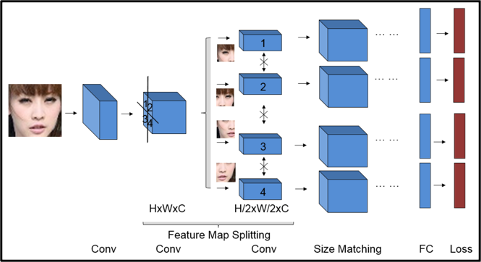
\includegraphics[scale=1]{image2-23-a}
  \label{image2-23-a}
\end{subfigure}
\begin{subfigure}{.5\textwidth}
  \centering
  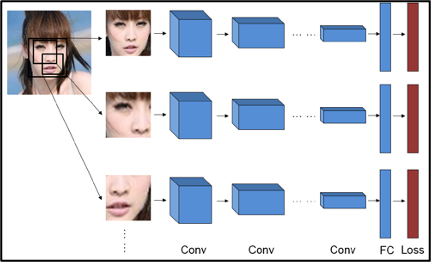
\includegraphics[scale=1]{image2-23-b}
  \label{image2-23-b}
\end{subfigure}
  \caption{ (الف) شبکه عصبی پیچشی \lr{SplitNet}  (ب) شبکه عصبی پیچشی معمولی \cite{ref1}.}
\label{fig:image2-23}
\end{figure}

\subsubsection{	شبکه \lr{GoogLeNet}}
در سال 2015 \lr{Christian Szegedy} و همکاران در \cite{7298594} یک شبکه عصبی عمیق به نام \lr{GoogLeNet} ارائه دادند. همانطور که در شکل 2-24 مشاهده می‌شود، \lr{GoogLeNet} یک شبکه عصبی پیچشی با 22 لایه است که یکی از اولین معماری های شبکه عصبی پیچشی بود که از رویکرد کلی قرار دادن تعداد زیادی از لایه‌های پیچشی و رای گیری  در کنار هم در یک ساختار متوالی بدست آمد. نویسندگان این مقاله همچنین تأکید کردند که این مدل جدید، توجه قابل ملاحظه ای به مصرف حافظه و مصرف انرژی دارد، زیرا کنار هم چیدن تعداد زیادی لایه و فیلتر دارای هزینه محاسباتی و حافظه است که احتمال بيش‌برازاندن  را افزایش می‌دهد.
 
\begin{figure}[h]
\centering
  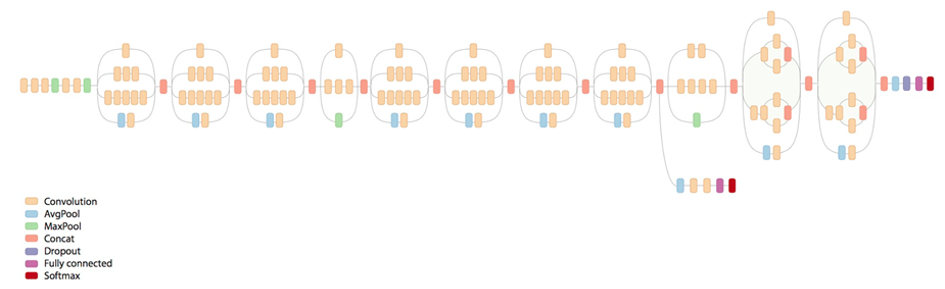
\includegraphics[scale=1]{image2-24}
  \caption{معماری کلی شبکه \lr{GoogLeNet} \cite{ref1}.}
  \label{image2-24}
\end{figure}

\noindent
در \lr{GoogLeNet} تمام محاسبات به طور متوالی اتفاق نمی‌افتد، بلکه هر بخش شبکه روندی موازی دارد. کادر سبز رنگ در شکل 2-25 بخش آغازگر نامیده می‌شود. در ادامه نگاهی دقیق تر به این بخش خواهیم داشت.
 
\begin{figure}[h]
\centering
  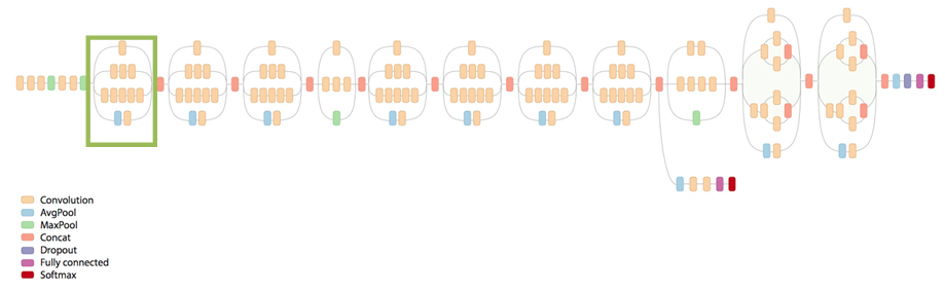
\includegraphics[scale=1]{image2-25}
  \caption{کادر سبز رنگ یکی از بخش های موازی شبکه را نشان می دهد \cite{ref1}.}
  \label{image2-25}
\end{figure}

\noindent
کادر سبز پایین در شکل 2-26 ورودی این بخش و کادر بالایی خروجی می‌باشد. در هر لایه شبکه‌های پیچشی معمولی، باید بین یک لایه پیچشی یا رای گیر، یکی را انتخاب نمود. در حالی که اینجا می‌توان تمام این عملیات را به صورت موازی انجام داد. این همان ایده ساده ای بود که نویسندگان مقاله روی آن تمرکز کردند.
 
\begin{figure}[h]
\centering
  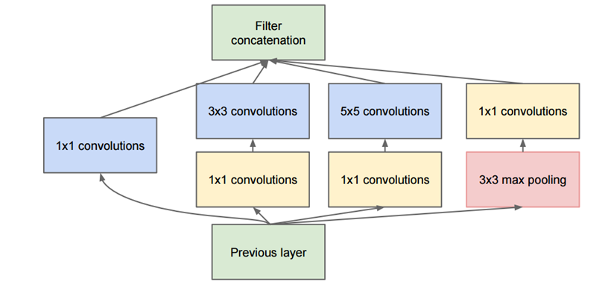
\includegraphics[scale=1]{image2-26}
  \caption{بخش آغازگر شبکه \lr{GoogLeNet} \cite{ref1}.}
  \label{image2-26}
\end{figure}

\subsubsection{	شبکه \lr{VGGFace}}
در سال 2015 \lr{Omkar M. Parkhi} و همکاران در \cite{parkhi2015deep} شبکه عمیق \lr{VGGFace} را ارائه کردند که شامل یک توالی طولانی از لایه‌های پیچشی می‌باشد. با توجه به شکل 2-27 این شبکه که در لایه آخر به عنوان یک طبقه‌بند عمل می‌نماید، هر تصویر آموزشی چهره را توسط لایه تماما متصل و تابع ضرر \lr{softmax log-loss} به یک بردار تبدیل می‌نماید که هر مقدار در این بردار، نشان دهنده احتمال برای یک هویت فردی است. \lr{VGGFace} مشابه \lr{FaceNet} از یک تابع ضرر سه گانه  در آموزش برای بهبود عملکرد کلی استفاده می‌نماید.
 
 \begin{figure}[h]
\centering
  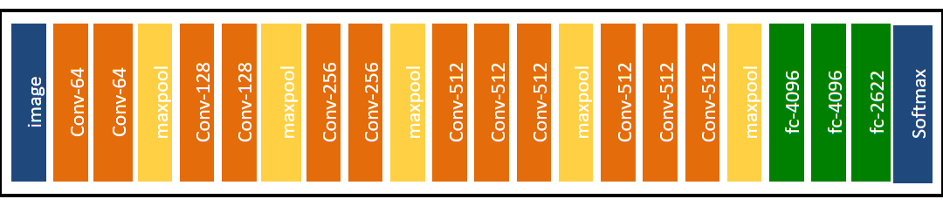
\includegraphics[scale=1]{image2-27}
  \caption{معماری شبکه \lr{VGGFace} \cite{ref1}.}
  \label{image2-27}
\end{figure}

 \subsection{رویکردهای مبتنی بر نقاط راهنما} 
چهره‌هايى كه در جهت‌هاى مختلفى هستند، براى سامانه تشخیص چهره، متفاوت به نظر مي‌رسند. براى غلبه بر اين چالش در رویکردهای مبتنی بر نقاط راهنما سعى مي‌شود تصوير را چرخانده و جابه جا نمود، بطوريكه چشم‌ها و لب‌ها در يك موقعيت خاص در تصوير قرار بگیرند. بدین ترتیب مقايسه چهره‌ها در مرحله بعد بسيار ساده‌تر خواهد شد.

\noindent 
در سال 2014 وحيد كاظمى و جوزفين ساليوان در \cite{6909637} یک الگوریتم برای یافتن نقاط راهنما بر روی چهره ارائه دادند كه از 194 نقطه خاص كه در هر چهره اى وجود دارد استفاده مي‌نماید. شکل 2-28 مکان این نقاط را بر روی گونه، لبه-هاى بیرونی چشم، كناره ابرو و... نشان می‌دهد. سپس اين 194 نقطه به سامانه آموزش داده می‌شود تا در هر چهره‌اى آن-ها را تشخيص دهد. 
\begin{figure}[h]
\centering
  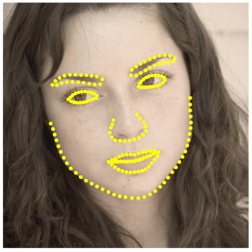
\includegraphics[scale=1]{image2-28}
  \caption{نتیجه موقعیت 194 شاخص روی چهره \cite{ref1}.}
  \label{image2-28}
\end{figure}

\noindent
پس از این که دانستیم چشم‌ها، دهان و ... کجاست، به راحتی می‌توانیم تناسب تصویر را تغییر داده و آن را چرخانده یا برش بزنیم. به طوری که چشم‌ها و دهان در بهترین حالت ممکن در مرکز قرار گیرد. با استفاده از تغییرات اساسی و اصلی تصویر، مانند تغییر اندازه، چرخش، خطوط موازی را حفظ می‌کنیم که در ریاضی به آن تغییرات نسبت یا افاین می‌گویند. شکل 2-29 علامت گذاری تکراری خطوط راهنما بر روی چهره را نشان می‌دهد. 
\begin{figure}[h]
\centering
  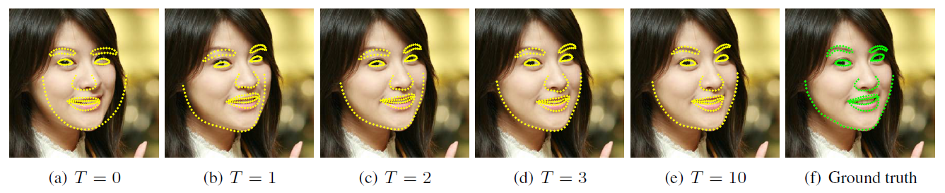
\includegraphics[scale=1]{image2-29}
  \caption{علامت گذاری خطوط راهنما بر روی چهره که در هر تکرار با کاهش خطا همراه می باشد \cite{ref1}.}
  \label{image2-29}
\end{figure}

\noindent
در سال 2016 \lr{Yue Wu} و همکاران در \cite{wu2016facial} رویکردی برای یافتن نقاط راهنما بر روی چهره مبتنی بر شبکه عصبی پیچشی ارائه دادند. در این مقاله یک معماری جدید برای شبکه عصبی پیچشی به نام
\lr{Tweaked CNN}
پیشنهاد شده است که به اختصار \lr{TCNN} نامیده می‌شود. این شبکه عصبی عمیق از 4 لایه پیچشی
(CL\textsubscript{1} … CL\textsubscript{4})
با لایه‌های رای‌گیری در میان آن‌ها تشکیل شده است و در انتهای یک لایه تمام متصل
FC\textsubscript{5}
و پس از آن یک لایه خروجی با اندازه
2×m
آمده است که مختصات \lr{m} نقطه ویژه را بر روی چهره مشخص می‌کند. در این مقاله \lr{m} برابر با 5 در نظر گرفته شده است. تابع فعالیت برای هریک از لایه‌های پیچشی
$f(x)=|tanh⁡(x)|$
 و تابع فعالیت برای لایه تمام متصل
$f(x)=tanh⁡(x)$
در نظر گرفته شده است. و در نهایت تابع زیر به عنوان تابع ضرر معرفی شده است.
\begin{equation}\label{eq2-12}
L(P_i,\hat{P_i})=\frac{(‖P_i-P ̂_i ‖_2^2)}{(‖P ̂_(i,1)-P ̂_(i,2) ‖_2^2 )}	
\end{equation}
که در آن
\lr{P\textsubscript{i}}
یک بردار
\lr{2×m}
برای مختصات پیش بینی شده تصویر
\lr{I\textsubscript{i}}
و
\lr{P\textsubscript{i}}
مختصات محل دقیق آن نقاط می‌باشد.
\lr{P\textsubscript{i,1}}
و
\lr{P\textsubscript{i,2}}
مختصات چشم ها در تصویر مرجع می‌باشند. در نهایت خروجی لایه تمام متصل توسط الگوریتم \lr{GMM} به 64 خوشه تقسیم شده و هریک به صورت جداگانه بررسی شده است. معماری \lr{TCNN} در شکل 2-30 قسمت b قابل مشاهده می‌باشد. این شبکه برای آموزش از مجموعه داده \lr{LFW} استفاده کرده است.
 
\begin{figure}[h]
\centering
  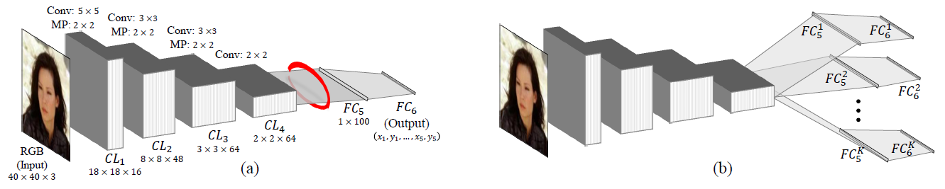
\includegraphics[scale=1]{image2-30}
  \caption{(a) شبکه عصبی پیچشی معمولی و (b) شبکه عصبی پیچشی با معماری \lr{TCNN} \cite{ref1}.}
  \label{image2-30}
\end{figure}

\section{جمع‌بندی}
در این فصل مفاهیم‌ پایه در مبحث یافتن و تشخیص چهره در تصاویر و انواع الگوریتم‌های دسته ‌بندی از روی تصاویر رنگی بررسی شد. همانطور که در قبل نیز بیان شد، برای حل مساله دسته ‌بندی چهره دو روش کلی، مبتنی بر تصویر و روش‌های مبتنی بر استخراج ویژگی وجود دارد. همچنین روش‌های مبتنی بر تصویر خود دارای رویکردهای مختلفی از جمله روش‌های مبتنی بر رنگ‌ بندی، روش‌های مبتنی بر شکل و روش‌های مبتنی بر گرادیان می‌باشد: همچنین روش های مبتنی بر استخراج ویژگی که در سال های اخیر بسیار مورد توجه قرار گرفته اند شامل رویکردهای مبتنی بر شبکه عصبی، بردار پشتیبان و... می باشند.